\documentclass[11pt,a4paper]{report}

\usepackage[utf8]{inputenc}
\usepackage[T1]{fontenc}
\usepackage[english]{babel}
\usepackage[top=2cm,bottom=2cm,left=1.5cm,right=2cm]{geometry}
%\usepackage{url}
%\usepackage{fancyhdr}
\usepackage{sectsty}
\usepackage{wrapfig}
\usepackage{titlesec}
\usepackage{setspace}
\usepackage{graphicx}
\usepackage{lmodern}
\usepackage{url}
\usepackage{amsmath}
\usepackage{amssymb}
\usepackage{mathrsfs}
\usepackage{fancyhdr}
\usepackage{gensymb}
\usepackage{enumerate}
\usepackage{hyperref} % Créer des liens et des signets 
\usepackage[cc]{titlepic}
\usepackage{caption}
\usepackage{verbatim}
\usepackage{color}
\usepackage{subfigure}
\usepackage{epsfig}
\usepackage{amsmath}
\usepackage{cancel}
\usepackage{enumitem}
\usepackage[justification=centering]{caption}
\setlist[enumerate]{font=\bfseries}
%\usepackage{euler}


\title{
\rule{15cm}{1pt} \\
\Large {\bfseries Intelligent mobile robotics} \\
\Large {\bfseries Assignment 3}\\
\rule{15cm}{1pt}}
\author{Sami Sellami}	

\titlepic{
\includegraphics[width=10cm]{Innopolis_image.PNG}} 
\date{\today}
 
\begin{document}
\pagenumbering{arabic}
\setcounter{page}{1}
\setcounter{secnumdepth}{1}
	
\fontfamily{ptm}\selectfont

\maketitle

\titlelabel{\thetitle)\quad}
\titlespacing{\chapter}{0cm}{0cm}{0cm}
\titlespacing{\section}{0.2cm}{0cm}{0cm}

\subsection{\textbf{Task1:}} 
The main objectif of the task is to implement an extended Kalman Filter in the case of robot localization and to design a relationship between the successive pose of a differential drive robot.\\
\begin{enumerate}
\item \textbf{The state variable vector of the robot:}\\
We choose as state vector for the differential drive robot the x, y positon wrt the world coordiante frame as well as the orientation $\theta$ of the robot frame wrt the world frame \ref{fig1}	
$$ x_{k} = \left[ \begin{array}{c} x\\ y\\ \theta \end{array}\right]$$ 

\begin{center}\label{fig1}
	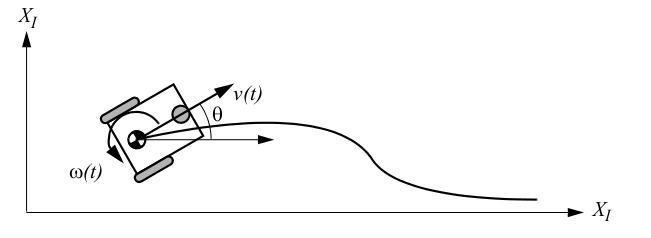
\includegraphics[width=8cm]{Capture1.png}
	\captionof{figure}{ {\small Movement of the differential drive robot}}	
\end{center}

\item \textbf{Designing the system model $\Phi_{k}$:}
For a differential-drive robot, the position can be estimated starting from a known position by integrating the movement (summing the incremental travel distances).
For a discrete system with a fixed sampling interval $\Delta t$ , the incremental travel distances are:
\begin{eqnarray}
\Delta x &= \Delta s \cdot \cos (\theta + \Delta \theta /2) \nonumber\\
\Delta y &= \Delta s \cdot \sin (\theta + \Delta \theta /2) \nonumber\\
\Delta \theta &= \dfrac{\Delta s_{r} - \Delta s_{l}}{b} \label{eq1}\\
\Delta s &= \dfrac{\Delta s_{r} + \Delta s_{l}}{2} \label{eq2}
\end{eqnarray}
Where : \qquad $ \left\{\ \begin{array}{l} \Delta x, \Delta y , \Delta \theta \qquad \textrm{path tavelled in the last sampling interval} \\
\Delta s_{l}  ,\Delta s_{r} \qquad \textrm{are the travelled distance for the left and right wheel respectively } \\
b \qquad \textrm{is the distace between two wheels of the differential drive robot}
\end{array}\right.  
$ 

Thus we get the motion model of the diffrential drive robot:
$$ \left [ \begin{array}{c} x_{k} \\ y_{k} \\ \theta_{k} \end{array}\right ]= 
\left [ \begin{array}{c} x_{k-1} \\ y_{k-1} \\ \theta_{k-1} \end{array}\right ] + 
\left [ \begin{array}{c} \Delta s \cdot \cos (\theta_{k-1} + \Delta \theta /2) \\ \Delta s \cdot \sin (\theta_{k-1} + \Delta \theta /2) \\ \Delta \theta \end{array}\right ]$$  

Using the relations \ref{eq1} and \ref{eq2} we find:
$$ \left [ \begin{array}{c} x_{k} \\ y_{k} \\ \theta_{k} \end{array}\right ]= 
\left [ \begin{array}{c} x_{k-1} \\ y_{k-1} \\ \theta_{k-1} \end{array}\right ] + 
\left [ \begin{array}{c} \dfrac{\Delta s_{r} + \Delta s_{l}}{2} \cdot \cos (\theta_{k-1} + \dfrac{\Delta s_{r} - \Delta s_{l}}{2b} ) \\ \dfrac{\Delta s_{r} + \Delta s_{l}}{2} \cdot \sin (\theta_{k-1} + \dfrac{\Delta s_{r} - \Delta s_{l}}{2b}) \\ \dfrac{\Delta s_{r} - \Delta s_{l}}{b} \end{array}\right ] = f(x, y, \theta) $$  

The control input is the actuation present on the wheels, however we consider that the motion velocity of the robot is constant so the input model is given by $ u = [\Delta s_{l} \quad \Delta s_{r}] = [v_{l} \cdot \Delta t \quad v_{r} \cdot \Delta t]$	

If we linearize the system with respect to the state vector we obtain the expression of $\Phi(x_{k})$  

$$ \Phi(x_{k}) =\nabla_{x} f=  \left [ \begin{array}{ccc} \dfrac{\partial f}{\partial x} & \dfrac{\partial f}{\partial y} & \dfrac{\partial f}{\partial \theta} \end{array}\right ] =
\left [ \begin{array}{ccc} 1 & 0 & -\Delta s \sin (\theta + \Delta \theta /2) \\ 0 & 1 & \Delta s \cos (\theta + \Delta \theta /2)\\ 0 & 0 & 1\end{array}\right ]  $$

\item \textbf{Obtaining the measurement model:}\\
We suppose that the position of the landmarks are given by $p_{x}^i$ and $p_{y}^i$, the position and orientation of the landmark relative to the robot is 
$$ \left \{\ \begin{array}{c} r^i= \sqrt{(p_{x}^i -x)^2 + (p_{y}^i -y)^2 } \\ \phi^i = \arctan (\dfrac{p_{y}^i - y}{p_{x}^i - x}) - \theta \end{array}  \right. $$ 

The measurement model is given by the expression :
$$ h^i (x_{k}^-)  = \left [ \begin{array}{c} \sqrt{(p_{x}^i -x)^2 + (p_{y}^i -y)^2 } \\ \arctan (\dfrac{p_{y}^i - y}{p_{x}^i - x}) - \theta \end{array}\right ] $$

Its linearization with respect to the state variables give the matrix $H^i$

$$ H^i = \left [ \begin{array}{ccc} \dfrac{-p_{x }^i+ x}{\sqrt{(p_{x}^i - x)^2 + (p_{y}^i-y)^2}}& \dfrac{-p_{y }^i+ y}{\sqrt{(p_{x}^i - x)^2 + (p_{y}^i-y)^2}} & 0 \\ 
 \dfrac{p_{y}^i - y}{(p_{x}^i - x)^2 + (p_{y}^i-y)^2}& \dfrac{x -p_{x}^i}{(p_{x}^i - x)^2 + (p_{y}^i-y)^2} & -1 
\end{array}  \right] $$ 

We assume that we have three landmarks positioned  like this:
\begin{align*}
p_{x}^1 &= 5 \qquad p_{y}^1 = 10\\
p_{x}^2 &= 10 \qquad p_{y}^2 = 5\\
p_{x}^3 &= 15 \qquad p_{y}^3 = 15
\end{align*}  
like that we will the final H matrix equal to 
$$ H =\left [ \begin{array}{ccc} H^1 \\H^2 \\H^3  \\H^4 \end{array}  \right] $$
 
\item\textbf{Writing the assumptions abouts the errors of the filter:}\\
The update covariance matrix of the extended Kalman filter is given by;
$$ P_{k}^- = \Phi_{k} P_{k} \Phi_{k}^T  + Q $$	
Where $P_{k-1}$ is the covariance of the previous robot state $x_{k-1}$ and $Q$ is the covariance of the noise associated to the motion model 
$$ Q = \nabla _{u}f \left [ \begin{array}{cc} k_{r}|\Delta s _{r}| & 0\\ 0 & k_{l} |\Delta s_{l}|\end{array} \right ] \nabla _{u}f^T $$
where $k_{r} $ and $k_{l}$ are error constants representing the nondeterministic parameters of the motor drive and the wheel floor interaction, to obtain this we make the assumption that error of the individually driven wheels are independant and that the variance of the error are proportional the absolute value of the travelled distace $\Delta s_{r} $, $\Delta s_{l}$
 
$$\nabla _{u} f = \left [\begin{array}{cc}  \dfrac{1}{2} \cos( \theta + \Delta \theta /2) - \dfrac{\Delta s}{2b}\sin(\theta + \Delta \theta /2) & \dfrac{1}{2} \cos( \theta + \Delta \theta /2) + \dfrac{\Delta s}{2b}\sin(\theta + \Delta \theta /2)\\
\dfrac{1}{2} \sin( \theta + \Delta \theta /2) + \dfrac{\Delta s}{2b}\cos(\theta + \Delta \theta /2) & \dfrac{1}{2} \sin( \theta + \Delta \theta /2) - \dfrac{\Delta s}{2b}\cos(\theta + \Delta \theta /2) \\
\dfrac{1}{b} & -\dfrac{1}{b} \end{array} \right] $$


We suppose also that the covariance matrix $P_{0}$ is known and equal to $P_{0} = \left [ \begin{array}{ccc} 0.2&0& 0 \\ 0 & 0.2 & 0\\ 0& 0& 1\end{array}\right ]$ also in our implementation, we approximate for simplicity the matrix Q as identity multiplied by a certain constant
 
After aquiring the sensors data , ie the position and orientation of the three landmarks, we need to compute the covariance matrix associated with each landmark, it can be approximated as 
$$ R^i = \left [ \begin{array}{cc} \sigma_{rr}^i & 0 \\ 0 & \sigma_{\phi \phi}^i\end{array} \right ] $$
We suppose  that the measurement of distance is independant from the orientation measurement , and for our code we take the following parameters $\sigma_{rr} =0.3 $ and $\sigma_{\phi\phi} = 0.1$ 

Thus the total covariance matrix for the whole set of landmarks should be like:
$$ R = \left [ \begin{array}{ccc} R^1 & 0 & 0 \\ 0 & R^2 & 0\\	
0 & 0 & R^3    \end{array} \right ] $$
 
\item \textbf{Drawing $P_{k}$ changes over time for two path(straight line and turn):} 
Applying the extended kalman Filter to our system means following the equation depicted below:
\begin{eqnarray}
x_{k}^- &=& f(x_{k-1}, u_{k}) \label{eq3}\\
P_{k}^- &=& P_{k} \Phi_{k} P_{k}^T  + Q \label{eq4}\\
K_{k} &=& P_{k}^- H_{k}^T (H_{k} P_{k}^-H_{k}^T  + R_{k})^-1 \label{eq5}\\
x_{k} &=& x_{k}^- +K_{k}(z_{k} - h(x_{k}^-)) \label{eq6}\\
P_{k} &=& (1 - K_{k}H_{k} ) P_{k}^-  \label{eq7} 
\end{eqnarray} 
 
After implementing the code and plotting the changes of the covariance matrix P over time we obtain the following graphs:
 
\begin{center}\label{fig2}
	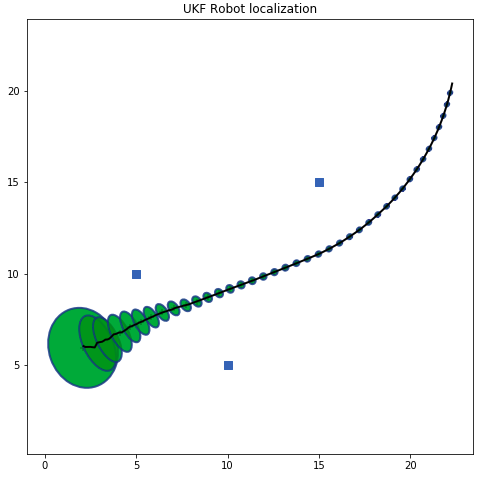
\includegraphics[width=8cm]{Capture2.png}
	\captionof{figure}{ {\small Pk changes over time}}	
\end{center}
 
To obtain this graph we set the commands of the robots ie the velocities of the right and left wheel equal in the first part of the trajectory and then set the right wheel velocity slightly greater than the left one, in a way that we obtaine the turn shown in the above picture. 
 
\subsection{\textbf{Task2:}}
In this task we are provided with a set of images where we need to locate a bounding box for an object that is moving, and extract some features points , the following figure shows the result for one keypoints that is plotted for 5 consecutive images     
\end{enumerate}

\begin{center}\label{fig2}
	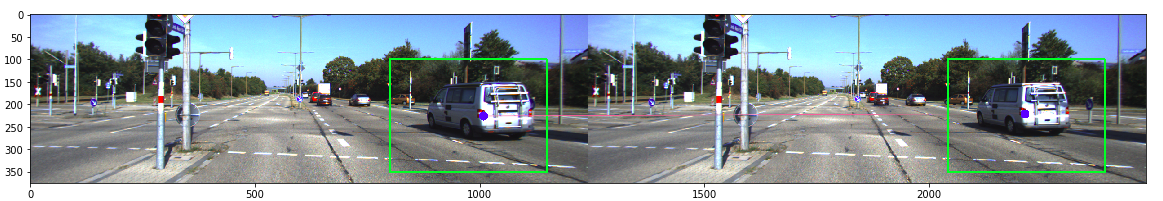
\includegraphics[width=17cm]{Capture3.png}\\
	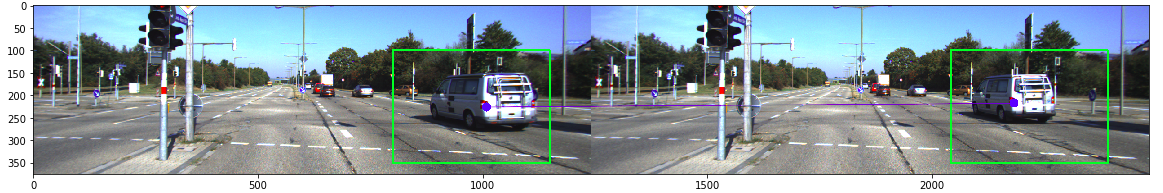
\includegraphics[width=17cm]{Capture4.png}\\
	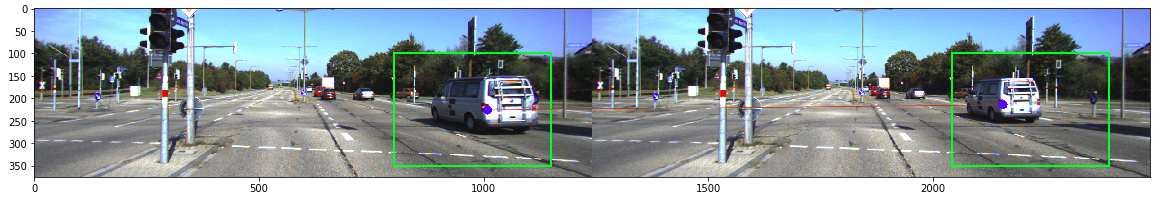
\includegraphics[width=17cm]{Capture5.png}\\
	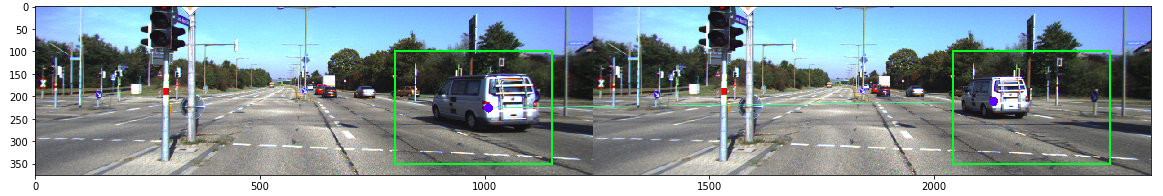
\includegraphics[width=17cm]{Capture6.png}
	\captionof{figure}{ {\small one keypoints in five consecutive images}}	
\end{center}
 
Then we suppose that the position of the robot is in the position of the keypoint aforementioned, after that, we need to extract landmarks to inject them in our EKF implementation, for this we extract new keypoints from the background and we consider them as landmarks, the following graph shows the keypoints extraction:
  
\begin{center}\label{fig3}
	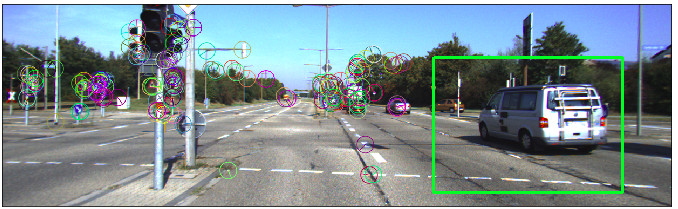
\includegraphics[width=15cm]{Capture8.png}\\
	\captionof{figure}{ {\small landmark extraction}}	
\end{center}

After injecting all this informations in our EKF implementation (initial position of the robot and the landmarks) we obtain the following graph showing of the trajectory of the robot(we suppose its moving on a straight line):

\begin{center}\label{fig4}
	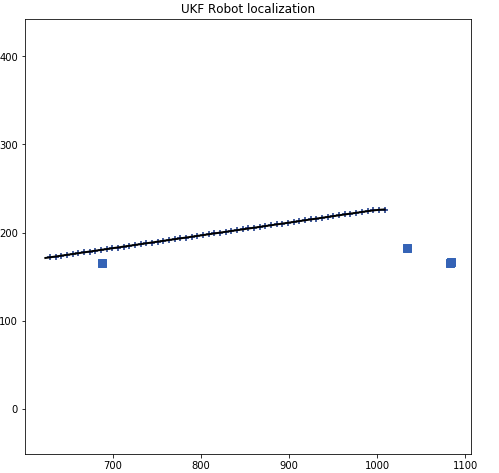
\includegraphics[width=7cm]{Capture9.png}\\
	\captionof{figure}{ {\small Trajectory estimation using extended kalman filter}}	
\end{center}



















 


  
\end{document}	
